\section*{Supplementary Note S1: F28379D Schedule and AFE Detail}

This note preserves the device-realistic implementation detail removed from the main manuscript during the v0.2 page-balance revision. It reports a simulation architecture and does not claim compiled firmware or bench validation.

\subsection*{S1.1 Register-realizable acquisition schedule}

The locked target is revision-C TMS320F28379D in the PTP-176 package. The system clock is 200~MHz, the ePWM clock is 100~MHz, and \texttt{TBPRD=1999} produces 50-kHz PWM. Four ADC modules operate in 16-bit differential mode at 50~MHz. With \texttt{ACQPS=63}, each aperture is 320~ns; acquisition plus conversion occupancy gives a 915-ns sustainable start interval, or 1.092896~MS/s per module.

The selected E1 rising-edge policy uses a 0.5-\si{\micro\second} guard and three points on each side of the reconstructed edge. Three start timestamps span 1.830~\si{\micro\second}, while their complete apertures span 2.150~\si{\micro\second}. Consequently, a 2.0-\si{\micro\second} point-timestamp-only design is a false pass. The locked ESR edge-fit window is $T_{w,R}=2.2$~\si{\micro\second} and retains 50~ns full-aperture margin. It is distinct from the $T_{w,C}=2.0$~\si{\micro\second} charge-safe window used by the capacitance observation and PE proof. Ten conversions per ADC per switching cycle correspond to 45.75\% utilization. Four DMA streams carry 4.0~MB/s in aggregate.

\begin{figure}[h]
\centering
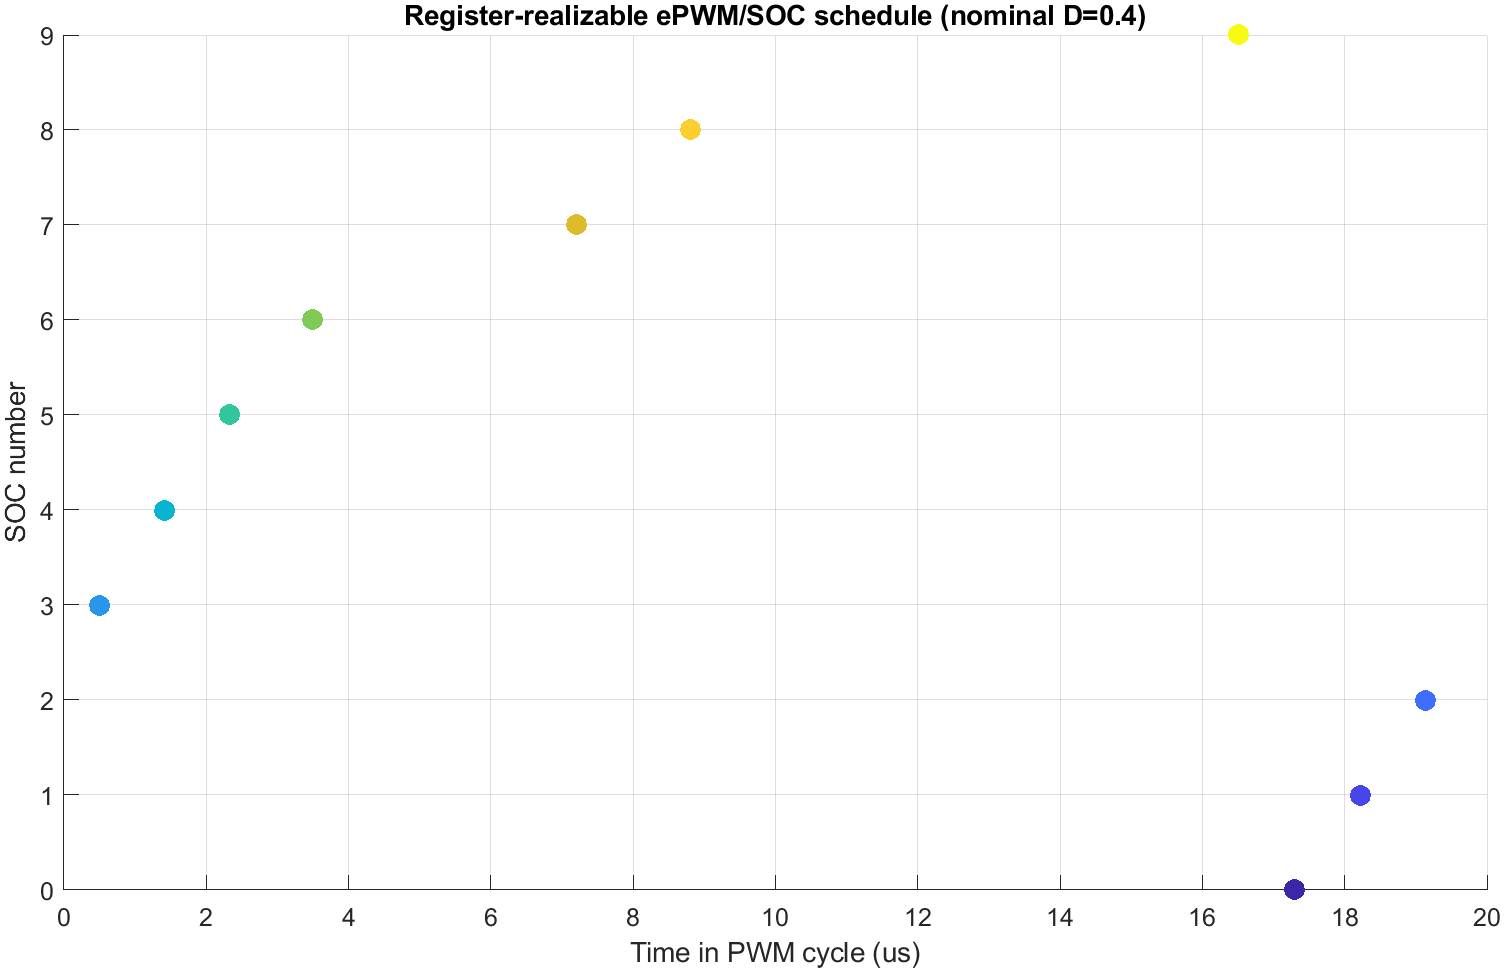
\includegraphics[width=0.95\linewidth]{figures/fig_f28379d_schedule.png}
\caption*{Fig. S1. Register-realizable one-edge ePWM/ADC schedule from the frozen v2.3 device study.}
\end{figure}

\begin{figure}[h]
\centering
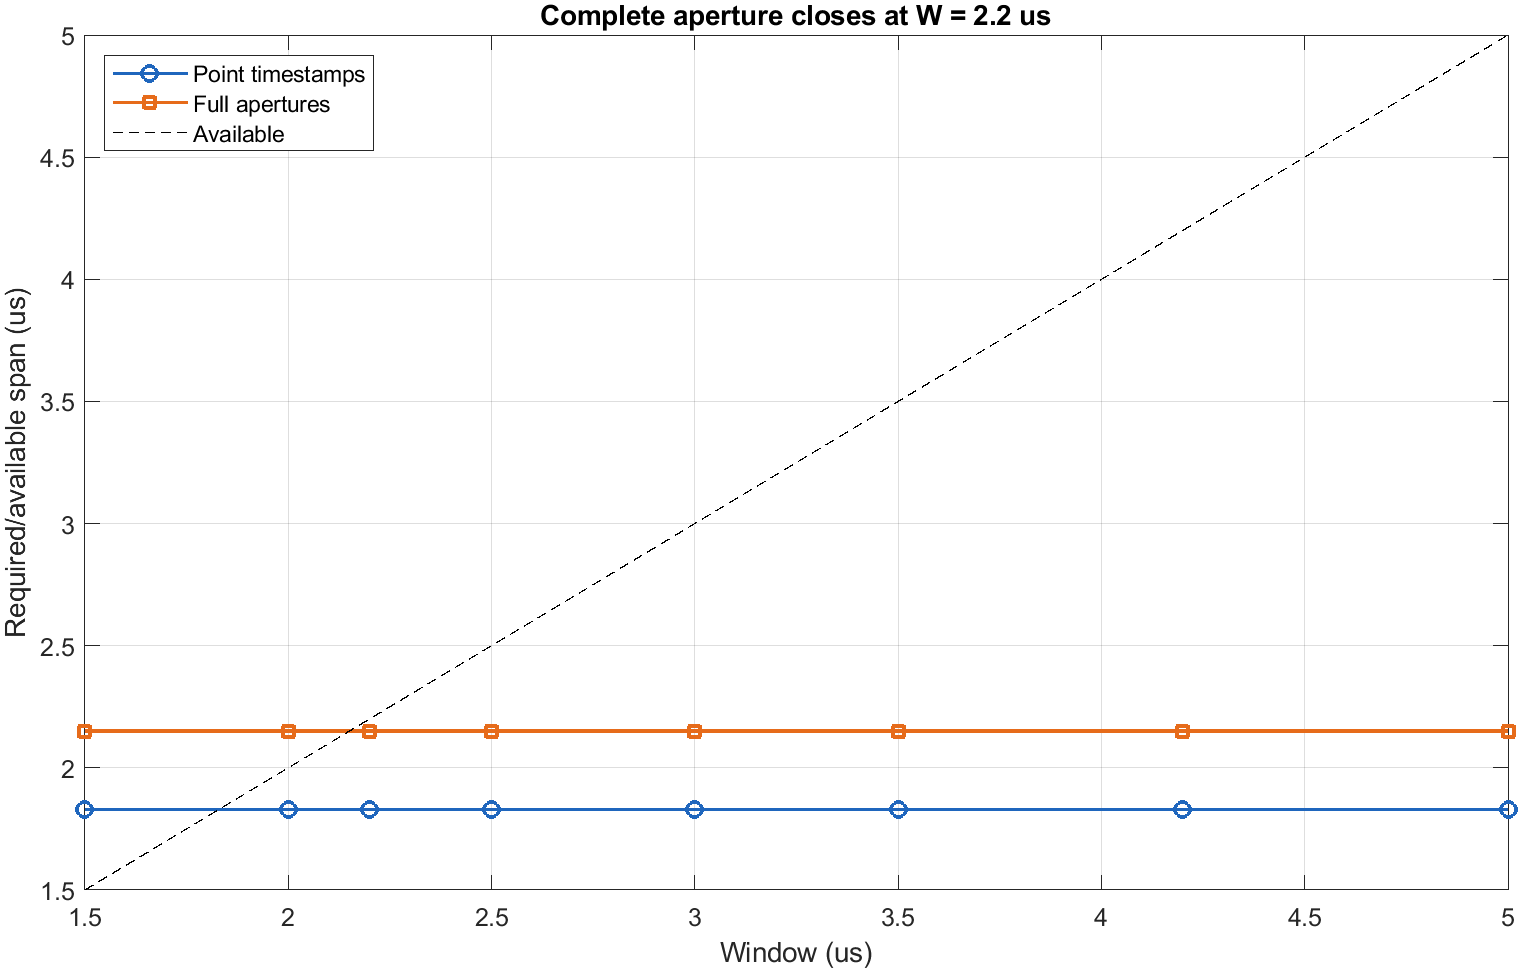
\includegraphics[width=0.72\linewidth]{figures/fig_f28379d_window.png}
\caption*{Fig. S2. Full-aperture edge-window geometry; the final sample aperture, not only its start time, lies inside the window.}
\end{figure}

\subsection*{S1.2 Differential AFE boundary}

The simulated capacitor-terminal common mode ranges from $-34.343$ to $+34.698$~V, whereas the differential ADC pins must remain between 0 and 2.5~V around a 1.25-V common mode. Direct connection is invalid. The declared AFE maps each channel to $V_P=1.25+V_{\mathrm{diff}}/2$ and $V_N=1.25-V_{\mathrm{diff}}/2$, with normal $|V_{\mathrm{diff}}|\le2.0$~V. The model uses source resistance no greater than 50~$\Omega$, a 330-pF reservoir on each pin, 1.2-MHz edge-path low-pass corner, edge-band CMRR at least 70~dB, and a synchronous common-mode template whose residual is no greater than 5\%.

Under those assumptions, the 0.5-\si{\micro\second} guard leaves 0.115\% calibrated settling residual and 1.72\% residual common-mode leakage relative to the weakest modeled ESR edge. Production multi-point calibration, external 2.5-V reference, and crystal/PLL are mandatory constraints. Failure to demonstrate them on the bench reopens the internal-ADC decision.

\subsection*{S1.3 Compute and validation boundary}

The conservative platform schedule assigns 4.5~\si{\micro\second} to DMA completion, 3.0~\si{\micro\second} to feature extraction, 5.0~\si{\micro\second} to estimator and integration work, and 1.5~\si{\micro\second} to diagnostics, leaving 6.0~\si{\micro\second} reserve in each 20-\si{\micro\second} PWM period. This 14-\si{\micro\second} allocation is a platform-level acquisition/processing budget; it must not be interpreted as the \TSRLS{} execution time. The separate frozen estimator-arithmetic estimate is 1.36~\si{\micro\second} per accepted observation, while external health reports are emitted every 1024 cycles (20.48~ms). Firmware was not compiled; linker placement and measured WCET are release gates. Seven representative device cases with 200 seeds each yielded worst p95 C/ESR endpoint errors of 1.6425\%/2.6109\%. Empirical 95\% interval coverage ranged from 93.5--97.5\% for capacitance and 98--100\% for ESR. These values remain device-realistic simulation results.

\begin{figure}[h]
\centering
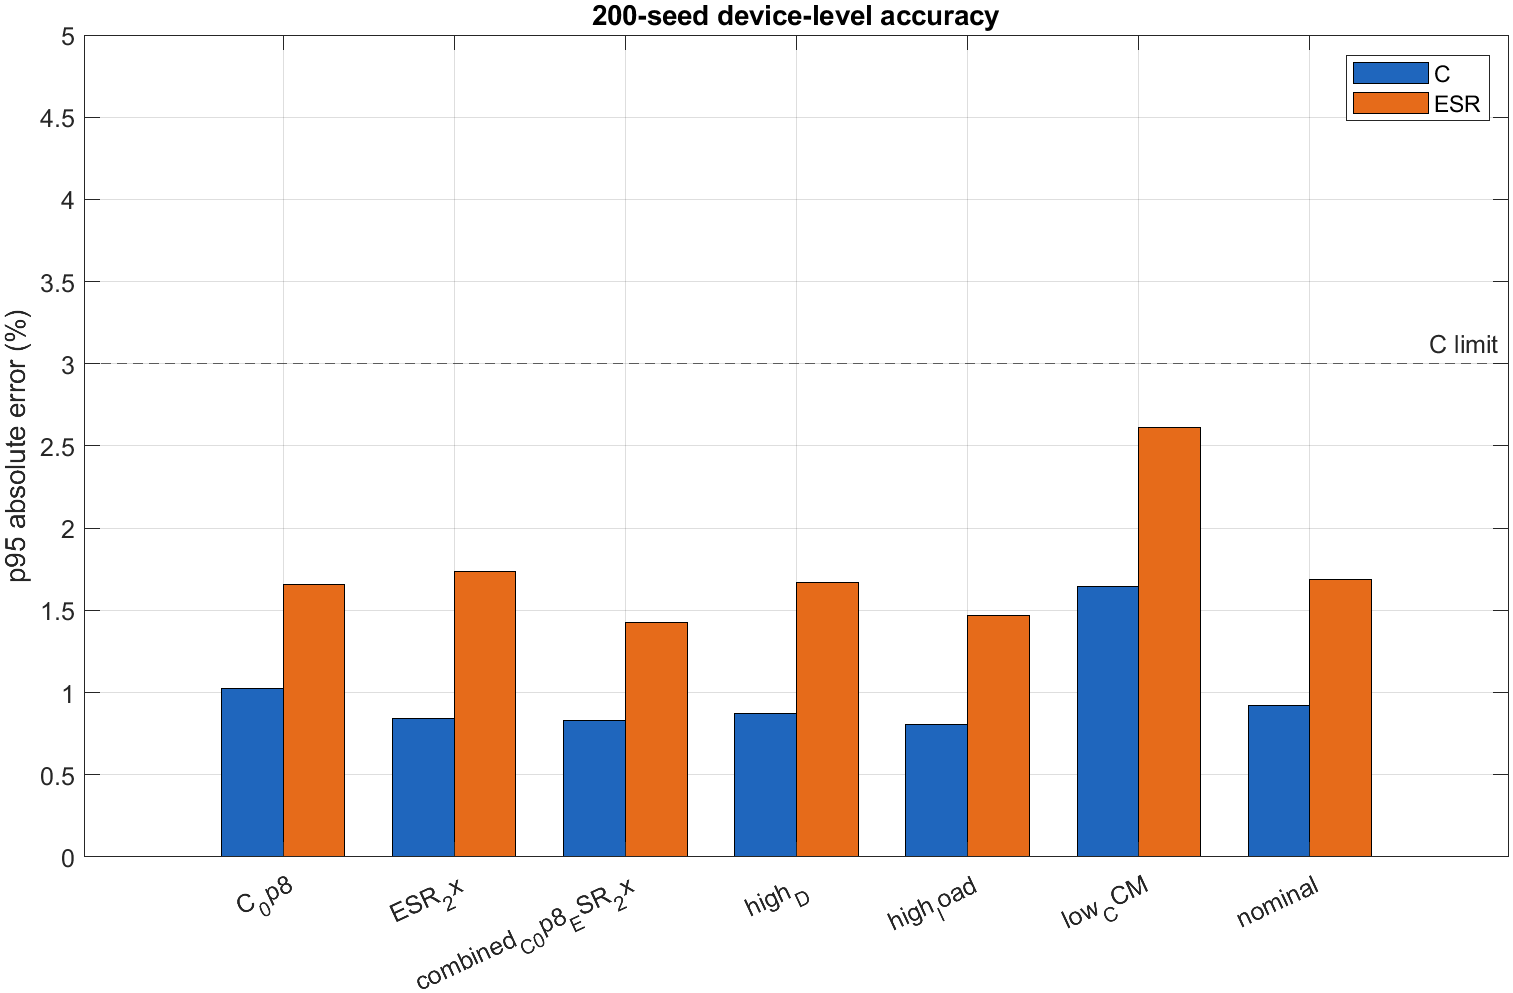
\includegraphics[width=0.78\linewidth]{figures/fig_f28379d_monte_carlo.png}
\caption*{Fig. S3. Device-realistic Monte Carlo endpoint-error summaries across the seven representative conditions.}
\end{figure}

\section*{Supplementary Note S2: $k_R$ Calibration Provenance}

This note records the closed edge-gain simulation-calibration provenance and the subsequent result regeneration. The archived v2.1 calibration chain was rerun from its source models, measurement-chain settings, and declared seeds. Each accepted edge supplies
\[
\kappa_m=\frac{z_{R,m}}{I_{\Sigma,m}r_{C,\mathrm{ref},m}},
\qquad
\hat k_R=\operatorname{median}_m\kappa_m.
\]
The reference ESR is the planted Model-A/Model-B simulation parameter. The implementation pools 147 finite ratios from each of four profiles and applies an unweighted median; its only omission rule is \texttt{NaN} removal. The resulting 588-ratio median exactly reproduces the archived v2.1 lock. Following the project decision, this full-precision value replaced the historical 0.982 campaign center, and all affected ESR results were regenerated with unchanged algorithms, hyperparameters, cases, and seeds.

\begin{table}[h]
\caption*{Table S2. $k_R$ calibration provenance}
\centering
\footnotesize
\begin{tabular}{p{4.2cm}p{7.0cm}}
\toprule
Item & Value \\
\midrule
Calibration source & Archived v2.1 Model-A/Model-B simulation calibration \\
Reference ESR & \texttt{SIMULATION\_REFERENCE\_TRUTH}, 0.05~$\Omega$ per calibration profile \\
Operating profiles & nominal; high duty/load; high noise; nominal Model-B with 10-nH ESL \\
Seeds & 11901--11904 \\
Accepted ratios & 588 (147 per profile) \\
Rejection rule & omit \texttt{NaN}; no residual rejection or trimming \\
Weighting & none \\
Aggregation & median of pooled $z_R/(I_\Sigma r_{C,\mathrm{ref}})$ ratios \\
Reproduced v2.1 value & 0.97719802594550731 \\
Archived v2.1 lock & 0.97719802594550731 \\
Recalibrated paper center & 0.97719802594550731 \\
Historical superseded center & 0.982 \\
Rerun scope & 4608-row factorial; static/dynamic algorithm-selection campaigns \\
Classification & \texttt{EXACT\_REPRODUCTION\_ADOPTED} \\
\bottomrule
\end{tabular}
\end{table}

The v1.1 evaluated proof constant $k_{R,\min}^{\mathrm{eval}}=0.957654065426597$ is $0.98$ times the archived v2.1 coefficient. It is a conservative evaluated-envelope lower bound and is not an online calibration value.

A separate 35-row residual-calibration-sensitivity check used five representative O1 cases, no retuning, and assumed gain errors from $-1\%$ to $+1\%$. Mean endpoint ESR bias ranged from $+1.0225\%$ at $-1\%$ gain error to $-0.9779\%$ at $+1\%$; the worst absolute case was $1.1708\%$. Unlike the casewise $\pm0.006$ variation in the main evaluation, this check represents residual unknown calibration error. It follows the inverse-scale relation while retaining finite observation noise. The later full rerun adopted the reproduced center rather than using the sensitivity study as an optimization.



